% Using KOMA Script document style
% Font size setting and
% option to skip empty lines as new paragraphs
\documentclass[10pt,a4paper]{article}
% Packages without Options
\usepackage{
	algorithm,
	algpseudocode,
	amsfonts,
	amssymb,
	appendix,
	array,
	booktabs,
	enumitem,
	float,
	footnote,
	gensymb,
	geometry,
	graphicx,
	interval,
	karnaugh-map,
	lipsum,
	listings,
	longtable,
	makecell,	mathtools,
	minted,
    nicematrix,
	parskip,
	pdfpages,
	pgfkeys,
	pgfplots,
    sectsty,
	subcaption,
	tablefootnote,
	textcomp,
	tikz,
    titlecaps,
	venndiagram,
	wrapfig,
	wrapfig,
	xcolor
}

% Packages with Options

\usepackage[framemethod=tikz]{mdframed}
\usepackage[colorlinks,linkcolor=cyan, citecolor=cyan, urlcolor=cyan]{hyperref}
\usepackage[labelfont=bf,textfont=it,labelsep=period]{caption}
\usepackage[RPvoltages]{circuitikz}
\usepackage[british]{babel}
\usepackage[nameinlink,noabbrev]{cleveref}

\definecolor{mintedbackground}{rgb}{0.97,0.97,0.97}

\setminted[cpp]{
bgcolor=mintedbackground,
    linenos=true,
    breaklines=true,}

\setminted[js]{
bgcolor=mintedbackground,
    linenos=true,
    breaklines=true,}

\setminted[python]{
bgcolor=mintedbackground,
    linenos=true,
    breaklines=true,}
    
% Enforce title case for section
\allsectionsfont{\titlecap}

% \lstset{basicstyle=\footnotesize\ttfamily,breaklines=true}

\linespread{1.5}



% Package: Interval
% Sets the style of mathematical intervals
\intervalconfig{
soft open fences, separator symbol=,,
}

% Package: Geometry
% Sets the page margins
\geometry{
    a4paper,
    left=32mm,
    right=22mm,
    top=22mm,
    }
	
% Creates a proper caption name for algorithms
\newcommand{\algorithmautorefname}{Algorithm}
\newcommand{\listingautorefname}{Listing}
\algrenewcommand{\algorithmiccomment}[1]{\texttt{// #1} }
% Creates a numbered environment for Theorems
\newtheorem{theorem}{Theorem}

% Redefine the implication arrow to be a simple, thin arrow instead of the default, thick arrow
\renewcommand{\implies}{\rightarrow}

% Create a new command for the set complement to make my logical statements easier to read
\newcommand{\compl}{\overline}

% Creates commands for combinatorics nCr and nPr
\newcommand{\nCr}[2]{\,_{#1}C_{#2}} % nCr
\newcommand{\nPr}[2]{\,_{#1}P_{#2}} % nPr

% Package: tikz
% Loads libraries for drawing automata, 
\usetikzlibrary{automata,positioning,shadows,arrows, shapes.gates.logic.US, calc}

% Creates a command to create a button shape
\newcommand*\keystroke[1]{%
  \tikz[baseline= (key.base)]
    \node[%
      draw,
      fill=white,
      drop shadow={shadow xshift=0.25ex,shadow yshift=-0.25ex,fill=black,opacity=0.75},
      rectangle,
      rounded corners=2pt,
      inner sep=1pt,
      line width=0.5pt,
      font=\scriptsize\sffamily
    ] (key) {#1\strut};
}

% Package: pgfplot
% Sets the global options for PGF Plots
\pgfplotsset{compat=newest}

% Package: tikz
% Flowchart Shapes
\tikzstyle{startstop} = [rectangle, rounded corners, minimum width=3cm, minimum height=1cm,text centered, draw=black, fill=red!30]
\tikzstyle{io} = [trapezium, trapezium left angle=70, trapezium right angle=110, minimum width=3cm, minimum height=1cm, text centered, draw=black, fill=blue!30]
\tikzstyle{process} = [rectangle, minimum width=3cm, minimum height=1cm, text centered, draw=black, fill=orange!30]
\tikzstyle{decision} = [diamond, minimum width=3cm, minimum height=1cm, text centered, draw=black, fill=green!30]
\tikzstyle{arrow} = [thick,->,>=stealth]

% Disable Minted syntax error highlights (red boxes)
\AtBeginEnvironment{minted}{%
  \renewcommand{\fcolorbox}[4][]{#4}}


\graphicspath{{images/}}

\title{CM1020: Discrete Mathematics \\ Summary}
\author{Arjun Muralidharan}
\begin{document}

\maketitle
\newpage
\tableofcontents
% \listoffigures
% \listoftables
% \listoflistings
% \listofalgorithms

\newpage
\renewcommand{\subsubsectionautorefname}{section\negthinspace}

\section{Sets}
\begin{mdframed}
\textbf{Learning Outcomes}
\begin{itemize}[label={\( \checkmark \)}]
\item Understand sets and power sets
\item Learn the listing methods and rules of inclusion methods
\item Learn to manipulate set operations
\item Represent a set using Venn diagrams
\item Understand and apply De Morgan’s law
\item Understand, and apply commutative, associative and distributive laws
\end{itemize}
\end{mdframed}

\subsection{Definition of a Set}
A set is an \emph{unordered collection} of \emph{distinct objects}, called \emph{elements}. We write \(	a \in A\) to denote that a is an element of the set A, and \(a \notin A\) to denote that a is \textbf{not} an element of A.

We can describe a set using \textbf{roster method} as \(A = \{a,b,c,d.\} \) or \textbf{set builder notation}: \[ A = \{ x \in \mathbb{Z} \mid x \textrm{ is odd} \} \]
Two sets are considered equal if they have the same elements.

\[
\forall x(x \in A \leftrightarrow x \in B)
\]
An empty set is denoted as \( \{ \} \) or \( \emptyset \). Do not confuse \( \emptyset \) with \( \{ \emptyset \} \) (the set containing the empty set).

\subsection{Subsets}
\(A\) is a subset of \(B\) if and only if all elements of A are in B. B is a superset of A.
\begin{gather*}
		A \subseteq B \\
	B \supseteq A
\end{gather*}

Further, we can show \textbf{proper subsets}, which imply that A \(\neq \) B
\begin{gather*}
		A \subset B \\
	B \supset A
\end{gather*}

\paragraph{Show that \(A \subseteq B\)} Show that if \(x\) belongs to \(A\), then \(x\) belongs to \(B\).
\paragraph{Show that \(A \not\subseteq B\)} Find a single \(x \in A\) such that \(x \notin B\)
\paragraph{Show that \(A = B\)} Show that \(A \subseteq B\) and \(B \subseteq A\)

Every nonempty set \(S\) has at least two subsets: the empty set \( \emptyset \) and the set \(S\) itself.

\subsection{Cardinality}
The \emph{cardinality} of a \emph{finite }set \(S\) is denoted as \(| S |\) and describes the number of distinct elements in a set. Because the empty set has no elements, it follows that \(| \emptyset | = 0\).

\subsection{Power Sets}
The power set \(\mathcal{P}(S)\) of \(S\) is the set of all subsets of the set \(S\). For nonempty sets, the empty set and the set itself are members of the power set.

The empty set has exactly one subset, itself.
\[
\mathcal{P}(\emptyset) = \{ \emptyset \}
\]
The set \( \{ \emptyset \} \) has two subsets.
\[
\mathcal{P}(\{ \emptyset \}) = \{ \{ \emptyset \}, \emptyset \}
\]
If two sets have the same power set, the sets themselves are equivalent. That is:
\[
	\mathcal{P}(A) = \mathcal{P}(B) \leftrightarrow A = B
\]

The cardinality of a power set is given as
\begin{equation*}
|\mathcal{P}(S)|= 2^n \textrm{ where } n \textrm{ is the cardinality of }S
\end{equation*}

\subsection{Set Operations \& Identities}
The Universal Set is denoted as \(U\) and contains everything.

\subsubsection{Union} The union of \(A\) and \(B\) is denoted as \(A \cup B \) and contains all elements that are in \(A\) or \(B\), or both. This is shown in \autoref{fig:union}.
\[ 	A \cup B = \{x \mid x \in A \vee x \in B \} \]
\begin{figure}[ht]
\begin{center}
\begin{venndiagram2sets}
\fillA{} \fillB{}
\end{venndiagram2sets}
\caption{Union of two sets}\label{fig:union}
\end{center}
\end{figure}
The union of sets is \textbf{commutative}, \textbf{associative} and \textbf{distributive} over the intersection.
\begin{align*}
	A \cup B &= B \cup A  \tag{Commutative Property}\\
	(A \cup B) \cup C &= A \cup (B \cup C)  \tag{Associative Property}\\
	A \cup (B \cap C) &= (A \cup B) \cap (A \cup C)  \tag{Distributive Property}
\end{align*}

\subsubsection{Intersection} The intersection of \(A\) and \(B\) is denoted as \(A \cap B \) and contains all elements that are in \(A\) and \(B\). This is shown in \autoref{fig:intersection}.
\[ A \cap B = \{x \mid x \in A \wedge x \in B \} \]
The intersection of sets is \textbf{commutative}, \textbf{associative} and \textbf{distributive} over the union.
\begin{align*}
A \cap B &= B \cap A \tag{Commutative Property}\\
(A \cap B) \cap C &= A \cap (B \cap C) \tag{Associative Property}\\
A \cap (B \cup C) &= (A \cap B) \cup (A \cap C)  \tag{Distributive Property}
\end{align*}
Two sets are called \emph{disjoint} if \(A \cap B = \emptyset \).

\begin{figure}[ht]
	\begin{center}
		\begin{venndiagram2sets}
		\fillACapB{}
		\end{venndiagram2sets}
		\caption{Intersection of two sets}\label{fig:intersection}
	\end{center}
\end{figure}
\subsubsection{Set Difference} The difference of \(A\) and \(B\) is denoted as \(A - B \) and contains all elements that are in \(A\) but not \(B\). This is shown in \autoref{fig:setdiff}.
\[
	A - B = \{x \mid x \in A \wedge x \notin B \}
\]
The set difference of sets is \textbf{not commutative} and \textbf{not associative}.
\begin{align*}
A - B &\neq B \cap B - A\\
(A - B) \cap C &\neq B - A
\end{align*}

An important identity for the set difference is \[
A - B = A \cap \overline{B}
\]
\textbf{Important:} The difference of two sets is not treated like an arithmetic subtraction. It only means taking all elements of a set, and removing any elements that overlap with the second set.
\begin{figure}[ht]
\begin{center}
\begin{venndiagram2sets}
\fillOnlyA{}
\end{venndiagram2sets}
\caption{Set difference of two sets}\label{fig:setdiff}
\end{center}
\end{figure}
\subsubsection{Complement} \(U\) is the universal set comprising everything. The complement of \(A\) with respect to \(U\) is denoted as \(\bar{A}\) and contains all elements that are in \(U\) but not \(A\). This is equivalent to \(U - A\) and is shown in \autoref{fig:setcompl}.
\[
	\bar{A} = \{x \mid x \in U \wedge x \notin A \}
\]
\begin{figure}[ht]
\begin{center}
\begin{venndiagram2sets}
\fillNotA{}
\end{venndiagram2sets}
\caption{Complement of a set}\label{fig:setcompl}
\end{center}
\end{figure}
\subsubsection{Symmetric  Difference} The symmetric difference of \(A\) and \(B\) is denoted as \(A \oplus B \) and contains all elements that are in \(A\) or in \(B\), but \textbf{not} in both. This is shown in \autoref{fig:symmdiff}.
\[
	A \oplus B = \{x \mid (x \in A \vee x \notin B ) \textrm{ and } x \notin A \cap B \}
\]
In other words, \(A \oplus B = A \cup B - A \cap B \).
\begin{figure}[ht]
\begin{center}
\begin{venndiagram2sets}
 \fillANotB{} \fillBNotA{}
 \end{venndiagram2sets}
\caption{Symmetric difference of two sets}\label{fig:symmdiff}
 \end{center}
\end{figure}

The symmetric difference of sets is \textbf{commutative} and \textbf{associative}. The intersection is \textbf{distributive} over the symmetric difference.

\begin{align*}
A \oplus B &= B \oplus A \tag{Commutative Property}\\
(A \oplus B) \oplus C &= A \oplus (B \oplus C) \tag{Associative Property}\\
A \cap (B \oplus C) &= (A \cap B) \oplus (A \cap C)  \tag{Distributive Property}
\end{align*}
\subsubsection{Cartesian Products}\label{sec:cart}
The \emph{ordered n-tuple \((a_1, a_2, \ldots, a_n)\)} is the ordered collection that has \(a_1\) as its first element, \(a_2\) as its second element, \ldots, and \(a_n\) as it \emph{n}th element.

Let \(A\) and \(B\) be sets. The \emph{Cartesian Product} of \(A\) and \(B\), denoted by \(A \times B\), is the set of all ordered pairs \((a, b)\) where \(a \in A\) and \(b \in B\). Hence, \[
	A \times B = {(a,b) \mid a \in A \wedge b \in B}
\]

\subsection{Principle of Inclusion-Exclusion }
When operating on the \emph{union}  of two or more sets, the cardinality of the union can be determined using the \textbf{principle of inclusion-exclusion}.

The cardinality of the union of two sets is given by adding the cardinalities of the two sets, and subtracting the cardinality of the intersection (as to not double count these elements).
\[	| A \cup B | = |A| + |B| - |A \cap B| \tag{Principle of inclusion-exclusion}\]

For three sets, the principle states that the ``undercount'' of elements must be added back.
\[	
  |A \cup B \cup C| = |A| + |B| + |C| - |A \cap B| - |A \cap C| - |B \cap C| + |A \cap B \cap C|
\]

More generally, the principle states that the cardinality of the union of \( n \) sets is given by \emph{adding}  the individual cardinalities, \emph{subtracting}  the cardinalities of the intersections of all pairs, \emph{adding}  the cardinalities of the intersection of all 3-tuple sets, \emph{subtracting}  the cardinalities of 4-tuple sets, and so on. Formally:

Let \( A_1, A_2, \ldots, A_n \) be finite sets. Then

\begin{align*}
  |A_1 \cup A_2 \cup \cdots \cup A_n| &= \sum_{1 \leq i \leq n} |A_i| - \sum_{1 \leq i \leq j \leq n} |A_i \cap A_j| \\ &+ \sum_{1 \leq i \leq j \leq k \leq n} |A_i \cap A_j \cap A_k| - \cdots + {(-1)}^{n+1} |A_1 \cap A_2 \cap \ldots \cap A_n|.
\end{align*}


\subsection{De Morgan's Laws}
De Morgan's laws describe how mathematical statements and concepts are related through their opposites.
\paragraph*{First Law} The complement of the union of two sets is equal to the intersection of their complements.

\[
\overline{A \cup B} = \overline{A} \cap \overline{B}
\]
\paragraph{Second Law} The complement of the intersection of two sets is equal to the union of their complements.

\[
	\overline{A \cap B} = \overline{A} \cup \overline{B}
\]

\subsection{Summary of Identity Laws}
A compiled overview of identity laws of sets are shown in \autoref{tab:identlawssets}.
\begin{table}[H]
\centering
\scriptsize
\def\arraystretch{1.4}
\begin{tabular}{p{0.4\textwidth}p{0.4\textwidth}}
\toprule
Name  & Identity \\ \midrule
\textbf{Identity Laws} & \(A \cap U = A\) \\
\textbf{} & \(A \cup \emptyset = A\) \\\midrule
\textbf{Domination Laws} & \(A \cup U = U\) \\
\textbf{} &  \(A \cap \emptyset = \emptyset \) \\\midrule
\textbf{Idempotent Laws} & \(A \cup A = A\) \\
\textbf{} &  \(A \cap A = A\) \\\midrule
\textbf{Complementation Law} & \(\overline{\overline{A}} = A \) \\\midrule
\textbf{Commutative Laws} & \( A \cup B = B \cup A \) \\
\textbf{} & \(A \cap B = B \cap A \) \\\midrule
\textbf{Associative Laws} & \((A \cup B) \cup C = A \cup (B \cup C)\) \\
\textbf{} & \((A \cap B) \cap C = A \cap (B \cap C) \) \\\midrule
\textbf{Distributive Laws} & \(A \cup (B \cap C) = (A \cup B) \cap (A \cup C) \) \\
\textbf{} & \(A \cap (B \cup C) = (A \cap B) \cup (A \cap C) \) \\
\textbf{} & \(A \cap (B \oplus C) = (A \cap B) \oplus (A \cap C)\) \\\midrule
\textbf{De Morgan's Laws} & \(\overline{A \cup B} = \overline{A} \cap \overline{B}
 \) \\
\textbf{} & \(\overline{A \cap B} = \overline{A} \cup \overline{B}\) \\\midrule
\textbf{Absorption Laws} & \(A \cup (A \cap B) = A \) \\
\textbf{} & \(A \cap (A \cup B) = A \) \\\midrule
\textbf{Complement Laws} & \(A \cup \overline{A} = U \) \\
\textbf{} & \(A \cap \overline{A} = \emptyset \) \\ \bottomrule
\end{tabular}
\caption{Summary of Identities in Set Theory}\label{tab:identlawssets}
\end{table}

\subsection{Partitions}
A \textbf{partition} of a set \(S\) is a a set of \emph{disjointed, non-empty} subsets of \(S\) that have \(S\) as their union. This is shown in \autoref{fig:partition}.
\begin{figure}[H]
\centering
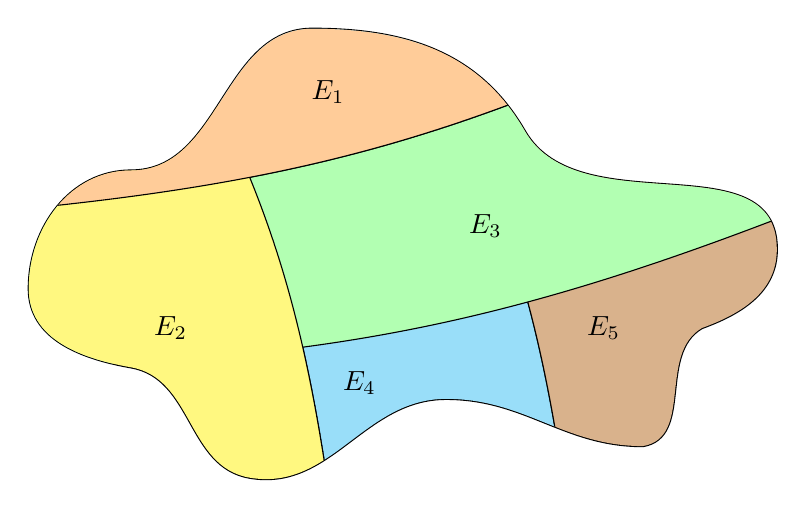
\begin{tikzpicture}

\path
  coordinate (aux0) at (0,1.5)
  coordinate (aux1) at (0,3.5)
  coordinate (aux2) at (10,3.5)
  coordinate (aux3) at (9,6)
  coordinate (aux4) at (4,0)
  coordinate (aux5) at (7,0)
  coordinate (aux6) at (2,6)
  coordinate (aux7) at (5,6)
  coordinate (esp1) at (0.2,2.5)
  coordinate (esp2) at (1.5,1.5)
  coordinate (esp3) at (3,0.1)
  coordinate (esp4) at (5.5,1.1)
  coordinate (esp5) at (8,0.5)
  coordinate (esp6) at (8.75,2)
  coordinate (esp7) at (9.7,3)
  coordinate (esp8) at (6.5,4.5)
  coordinate (esp9) at (3.8,5.8)
  coordinate (esp10) at (1.5,4)
  ;
\draw[line width=0.8pt]
  (esp1) to[out=-90,in=170]
  (esp2) to[out=-10,in=170]
  (esp3) to[out=-10,in=180]
  (esp4) to[out=0,in=180]
  (esp5) to[out=10,in=-150]
  (esp6) to[out=20,in=-90]
  (esp7) to[out=90,in=-60]
  (esp8) to[out=120,in=0]
  (esp9) to[out=180,in=0]
  (esp10) to[out=180,in=90]
  cycle;
\clip
  (esp1) to[out=-90,in=170]
  (esp2) to[out=-10,in=170]
  (esp3) to[out=-10,in=180]
  (esp4) to[out=0,in=180]
  (esp5) to[out=10,in=-150]
  (esp6) to[out=20,in=-90]
  (esp7) to[out=90,in=-60]
  (esp8) to[out=120,in=0]
  (esp9) to[out=180,in=0]
  (esp10) to[out=180,in=90]
  cycle;
\filldraw[fill=cyan!40]
  (aux4) to[bend right=10]
  (aux6) --
  (aux7) to[bend left=10]
  (aux5) -- cycle;
\filldraw[fill=brown!60]
  (aux5) to[bend right=10]
  (aux7) --
  (10,6) --
  (10,0) -- cycle;
\filldraw[fill=green!30]
  (aux0) --
  (aux1) to[bend right=10]
  (aux3) --
  (10,6) --
  (aux2) to[bend left=10] cycle;
\filldraw[fill=yellow!50]
  (0,0) --
  (aux4) to[bend right=10]
  (aux6) --
  (0,6) --
  (0,0) -- cycle;
\filldraw[fill=orange!40]
  (0,6) --
  (aux1) to[bend right=10]
  (aux3) --
  (0,6) -- cycle;
\node at (4,5) {$E_1$};
\node at (2,2) {$E_2$};
\node at (6,3.3) {$E_3$};
\node at (4.4,1.3) {$E_4$};
\node at (7.5,2) {$E_5$};
\end{tikzpicture}
\caption{Partitions of a set}\label{fig:partition}
\end{figure}

In other words, the set of subsets \(A_i\) is a partition of \(S\) if and only if
\begin{gather*}
	A_i \neq \emptyset \\
	A_i \cap A_j = \emptyset \mathrm{ when } i \neq j \\
A_1 \cup  A_2 \cup A_3 \ldots \cup A_i = S
\end{gather*}

\section{Functions}\label{sec:functions}
\begin{mdframed}
\textbf{Learning Outcomes}
\begin{itemize}[label={\( \checkmark \)}]
\item Understand what is a function and define its domain, and co-domain,
\item Define the range of a function and the pre-image of an element
\item Recognise linear, quadratic and exponential functions
\item Define and learn examples of injective and surjective functions.
\item Build functions compositions and a function’s inverse.
\item Recognise and define some particular functions such as absolute value, floor, ceiling
\end{itemize}
\end{mdframed}
\subsection{Definition of a function}

Let \(A\) and \(B\) be nonempty sets. A \emph{function} from \(A\) to \(B\) is an assignment of exactly one element of \(B\) to every element of \(A\). That is, \textbf{every pre-image has exactly one image} (many-to-one). \[
  f\colon A \rightarrow B
\]
A function is a subset of the cartesian product (see \autoref{sec:cart}) \(A \times B\) that has only one ordered pair \((a,b)\) for each \(a \in A\).

\subsection{Domain, Co-Domain and Range}\label{ssub:domain_co_domain_and_range}
In a function \(f\colon A \rightarrow B\), \(A\) is the \textbf{domain} \(D_f\), and \(B\) is the \textbf{co-domain} \(Co\text{-}D_f\). When noted as \(f(a) = b\), \(a\) is the \emph{pre-image} and \(b\) is the \emph{image}. The \textbf{range} \(R_f\) is the set of all images of \(A\) in \(B\).

Two functions are \emph{equal} if and only if they have the same domain, co-domain and map each element of the domain the same element in the co-domain.

A function is called \emph{real-valued} if \(D_f = \mathbb{R}\) and \emph{integer-valued} if \(D_f = \mathbb{Z} \).

\subsection{Injective \& Surjective Functions}\label{ssub:injective_&_surjective_functions}
\subsubsection{Injective Functions}\label{ssub:injective_functions}


A function is \textbf{injective} (or one-to-one) if \(f(a) = f(b) \rightarrow a = b\). In other words, if two images are the same, their pre-images are the same. \textbf{Every image has  exactly one pre-image or isn't assigned to a pre-image}. In other words, every image has no more than one pre-image. This is clarified by the contrapositive of the above implication: \(f(a) \neq f(b) \rightarrow a \neq b \). In general: \[
  \forall a \forall b(a = b \rightarrow f(a) = f(b))
\]

If a function is \textbf{strictly increasing} or \textbf{decreasing} (i.e. \( \forall a \forall b(a \leq b \rightarrow f(a) \leq f(b)) \) or \( \forall a \forall b(a \geq b \rightarrow f(a) \geq f(b)) \)), the function is injective.

\paragraph{Proof} To prove a function is injective, show that for a fixed \( x_1, x_2 \in D_f \)  where  \( f(x_1) = f(x_2)\) it follows that \( x_1 = x_2 \). This can be done by transforming the equation \( f(x_1) = f(x_2) \) to the form \( x_1 = x_2 \)  

\subsubsection{Surjective Functions}\label{ssub:surjective_functions}
A function is \textbf{surjective} (or onto) if \(\forall y \exists x(f(x) = y)\). That is, \textbf{for every image in \(Co\text{-}D_f\) there exists a pre-image in \(D_f\)} , thus \(Co\text{-}D_f = R_f\).

\paragraph{Proof} To prove a function is surjective, express \( x \) in terms of \( y \)  and insert into the function \( f(x) \). Then, transform this to \( f(x) = y \) and confirm that there exists an \( f(x) \) for all \( y \) in the Co-Domain.

\subsection{Bijective Functions}
A function is called \emph{bijective} or a \emph{one-to-one correspondence} if it is \textbf{both injective and surjective}. 
\subsection{Inverse of a function}
The \textbf{inverse} \( f^{-1} \) of a \emph{bijective} function \(f:A \implies B \)  is the function that assigns a unique element of A to each element in B. Only bijective functions are \textbf{invertible}.

To find the inverse, transform the function \( f(x) \) to the form \( f(y) \), isolating x to one side.

\subsection{Composition}
The function composition of two functions \( f \) and \( g \) is denoted as \( f \circ g \). This is equivalent to first applying the right-most function (\( g \)), and subsequently applying the functions further upfront (\( f \)). \[
(f \circ g)(a) =  f(g(a))  
\]

The domain of the composition \( f \circ g \) is the domain of \( g \), while the co-domain is the co-domain of \( f \). Hence if \( f: A \implies B \) and \( g: B \implies C\) then \( f \circ g: A \implies C\). This is illustrated in \autoref{fig:composition}.

\begin{figure}[ht]
  \centering
  \includegraphics[width=\textwidth]{composition}
  \caption{The composition of functions \( f \) and \( g \)  }\label{fig:composition}
\end{figure}

\subsection{Floor and Ceiling Functions}
The \textbf{floor function} \(\lfloor x \rfloor \)  assigns to the real number \( x \) the largest integer that is less than or equal to \( x \).

The \textbf{ceiling function} \(\lceil x \rceil \)  assigns to the real number \( x \) the smallest integer that is greater than or equal to \( x \).
\section{Propositional Logic}
\begin{mdframed}
\textbf{Learning Outcomes}
\begin{itemize}[label={\( \checkmark \)}]
\item Define propositional logic and learn some of its properties 
\item Give some examples of domains where 
	propositional logic is used  
\item Defining a proposition in mathematical context and distinguish examples of sentences considered as propositions and other that are not propositions 
\item Learn how propositional variables help to simplify notations 
\item Learn how we can build a truth table and give an example of how it works 
\item Practice how to build compound statements using logical operators and take into consideration the order of precedence of the operators 
\item Define truth sets and learn some examples of truth sets for some compound propositions 
\item Define what is an implication and equivalence, what are their properties and build their truth table 
\item Learn some important laws of propositional logic including De Morgan’s laws, and practice their use in building a reasoning, and proving equivalence
\end{itemize}
\end{mdframed}
\subsection{Connectives}
A \textbf{proposition} is a declarative sentence that is either true or false, but not both. We use \textbf{propositional} or \textbf{sentential} variables such as \(p,q,r,s \ldots \) to represent propositions. The \textbf{truth value of a proposition} is denoted by \textbf{T} or \textbf{F}. The simplest form of a proposition is an \textbf{atomic proposition}. Propositions can be placed in relation to one another using \textbf{connectives}.

\subsubsection{Negation}
Let \( p \) be a proposition. The \emph{negation} of \(p\) is stated as \[\mathbf{\neg p}\]
and proposes that ``It is not the case that \(p\)''.

The proposition \(\neg p\) is read ``not \(p\)''. The truth value of the negation of \(p, \neg p, \) is the opposite of the truth value of \(p\).

\subsubsection{Conjunction}
Let \(p\) and \(q\) be propositions. The \emph{conjunction} of \(p\) and \(q\), is denoted as \[\mathbf{p \wedge q }\] and proposes that ``\(p\) and \(q\)''.

The \emph{conjunction} \(p \wedge q\) is true when both \(p\) and \(q\) are true and is false otherwise.

\subsubsection{Disjunction}
Let \(p\) and \(q\) be propositions. The \emph{disjunction} of \(p\) and \(q\), denoted as \[\mathbf{p \vee q }\] is the statement ``\(p\) or \(q\)''.

The \emph{disjunction} \(p \vee q\) is false when both \(p\) and \(q\) are false and is true otherwise. This is an \textbf{inclusive or}, which means that the disjunction is true if at least one of the propositions is true, or both are true.

\subsubsection{Conditional Statements \& Implication}
Let \( p \) and \( q \) be propositions. The \emph{conditional statement} \[
p \implies q	
\]
is the proposition ``if \( p \), then \( q \).'' The conditional statement \( p \implies q \) is false when \( p \) is true and \( q \) is false, and true otherwise. In the implication \( p \implies q \), \( p \) is the \emph{hypothesis} (or \emph{antecedent} or \emph{premise}) and \( q \) is called the \emph{conclusion} (or \emph{consequence}).

The implication does not express causality in discrete mathematics. It only covers the truth value of the statement. It can also be read as:

\begin{enumerate}
	\item ``\( p \) is sufficient for \( q \) ''
	\item ``a necessary condition for \( q \) is \( p \) ''
	\item ``\( q \) unless \( \neg p \) ''
	\item ``\( q \) whenever \( p \) ''
\end{enumerate}

\subsubsection{Exclusive Or}

Let \(p\) and \(q\) be propositions. The \emph{exclusive or} of \(p\) and \(q\), denoted as \[ \mathbf{p \oplus q }\] is the statement ``either \(p\) or \(q\), but not both''.

The \emph{exclusive or} \(p \oplus q\) is true when exactly one of \(p\) and \(q\) is true and false otherwise. In other words, \( p \) and \( q \) may never have the same truth value.  

\subsubsection{Biconditional}
Let \(p\) and \(q\) be propositions. The \emph{biconditional statement} \[ \mathbf{p \leftrightarrow q } \] is the proposition ``\(p\) if and only if \(q\)''.

The biconditional statement \(p \leftrightarrow q\) is true when \(p\) and \(q\) have the same truth values, and is false otherwise.

\subsection{Truth Tables}
A truth table evaluates the truth values for propositions and connectives systematically. When given a compound proposition, a truth table can be used to evaluate the atomic propositions step-by-step and arrive at the correct truth value for the compound proposition.

\begin{table}[H]
\centering
\caption{Truth table for basic connectives}\label{tab:truth}
\begin{tabular}{@{}>{\bfseries}c>{\bfseries}cccccc@{}}
\toprule
 \( \mathbf{p} \) & \( \mathbf{q} \) & \(p \wedge q\) & \(p \vee q\) & \(p \oplus q\) & \(p \implies q\) & \(p \leftrightarrow q\)  \\ \midrule
 T & T & T & T & F & T & T \\
 T & F & F & T & T & F & F \\
 F & T & F & T & T & T & F \\
 F & F & F & F & F & T & T \\
  \bottomrule
\end{tabular}
\end{table}
Truth values can also be denoted using binary bits, i.e.~T is 1 and F is 0. When constructing a truth table, the number of rows is \(2^n\) where n is the number of propositions involved. So compound proposition involving 3 atomic propositions \(p, q, r\) has \(2^3 = 8\) rows.
Further, The the first column (e.g.~\(p\)) is constructed with all true values for the first half, and false values for the second half, the second (\(q\)) is true for the first 2 rows and false for next two rows, and the third is true for the first row and false for the second row of the table, and then this pattern repeats down the table for \(p, q\) and \(r\).

The universal and existential quantifications \( \forall \) and \( \exists \) are described in \autoref{ssub:quantifiers}.

\subsection{Precedence of Logical Operators}
Logical operators have an order of precedence as follows. \[
\forall \quad \exists \quad \neg \quad \wedge \quad \vee \quad \implies \quad \leftrightarrow
\]
\subsection{Propositional Equivalences}\label{ssec:equiv}
\begin{enumerate}
	\item \textbf{Tautology:} A compound proposition that is always true, no matter the truth values of the individual propositions
	\item \textbf{Contradiction:} A compound proposition that is always false, no matter the truth values of the individual propositions. This is called \textbf{inconsistent}.
	\item \textbf{Contingency:} A compound proposition that is true for at least one scenario of truth values. This is called \textbf{consistent}. All tautologies are consistent by definition.
\end{enumerate}

% TODO: Add contrapositive comment to equivalences table

\subsection{Logical Equivalence}
Compound propositions that have the same truth value in all possible cases are called \textbf{logically equivalent}. In other words, if \(p \leftrightarrow q\) is a tautology, then \(p \equiv q\).

Logical equivalence can be proved using truth tables.

\subsection{De Morgan's Laws}
\begin{gather*}
\neg (p \wedge q) \equiv \neg p \vee \neg q  \tag{De Morgan's First Law} \\
\neg (p \vee q) \equiv \neg p \wedge \neg q \tag{De Morgan's Second Law}
\end{gather*}
\subsection{Special equivalences}
\subsubsection{Conjunction-Disjunction} The \textbf{conditional-disjunction equivalence} allows us to replace conditional statements with disjunctions. This is especially useful to convert a conditional to a form that can then be transformed using De Morgan's laws.

\begin{gather*}
p \implies q \equiv \neg p \vee q
\end{gather*}

\subsubsection{Contrapositive}The \textbf{contrapositive} of a conditional statement is equivalent to the original conditional statement and is defined as follows.
\begin{gather*}
p \implies q \equiv \neg q \implies \neg p
\end{gather*}

\subsection{Summary of Logical Equivalences}
\begin{table}[H]
\centering
\caption{Summary of Equivalence Laws}\label{tab:identlaws}
\def\arraystretch{1.4}
\begin{tabular}{p{0.4\textwidth}p{0.4\textwidth}}
\toprule
Name  & Equivalence \\ \midrule
\textbf{Identity Laws} & \(p \wedge \mathbf{T} \equiv p\) \\
\textbf{} & \(p \vee \mathbf{F} \equiv p\) \\\midrule
\textbf{Domination Laws} & \(p \vee \mathbf{T} \equiv \mathbf{T}\) \\
\textbf{} &  \(p \wedge \mathbf{F} \equiv \mathbf{F}\) \\\midrule
\textbf{Idempotent Laws} & \( p \vee p \equiv p \) \\
\textbf{} &  \(p \wedge p \equiv p\)  \\\midrule
\textbf{Double Negation Law} & \(\neg(\neg p) \equiv p\) \\\midrule
\textbf{Commutative Laws} & \( p \vee q \equiv q \vee p \) \\
\textbf{} & \(p \wedge q \equiv q \wedge p \) \\\midrule
\textbf{Associative Laws} & \( (p \vee q) \vee r \equiv p \vee(q \vee r) \) \\
\textbf{} & \((p \wedge q) \wedge r \equiv p \wedge(q \wedge r)\)  \\\midrule
\textbf{Distributive Laws} & \(p \vee(q \wedge r) \equiv(p \vee q) \wedge(p \vee r)\) \\
\textbf{} & \(p \wedge(q \vee r) \equiv(p \wedge q) \vee(p \wedge r)\) \\ \midrule
\textbf{De Morgan's Laws} & \(\neg(p \wedge q) \equiv \neg p \vee \neg q\) \\
\textbf{} & \(\neg(p \vee q) \equiv \neg p \wedge \neg q\) \\\midrule
\textbf{Absorption Laws} & \(p \vee(p \wedge q) \equiv p\) \\
\textbf{} & \(p \wedge(p \vee q) \equiv p\) \\\midrule
\textbf{Negation Laws} & \(p \vee \neg p \equiv \mathbf{T}\) \\
\textbf{} & \(p \wedge \neg p \equiv \mathbf{F}\) \\ \bottomrule
\end{tabular}

\end{table}
\subsubsection{Logical Equivalences Involving Conditional Statements}
\begin{align*}
p \implies q &\equiv \neg p \vee q \\
p \implies q &\equiv \neg q \implies \neg p\\
p \vee q &\equiv \neg p \implies q \\
p \wedge q &\equiv \neg(p \implies \neg q) \\
\neg(p \implies q) &\equiv p \wedge \neg q\\
(p \implies q) \wedge(p \implies r) &\equiv p \implies(q \wedge r) \\
(p \implies q) \wedge(q \implies r) &\equiv(p \vee q) \implies r \\
(p \implies q) \vee(p \implies r) &\equiv p \implies(q \vee r) \\
(p \implies r) \vee(q \implies r) &\equiv(p \wedge q) \implies r \\
(p \lor \neg r )\to (\neg q \land r)
\end{align*}

\subsubsection{Logical Equivalences Involving Biconditional Statements}
\begin{align*}
p \leftrightarrow q &\equiv(p \implies q) \wedge(q \implies p) \\ p \leftrightarrow q &\equiv \neg p \leftrightarrow \neg q \\ p \leftrightarrow q &\equiv(p \wedge q) \vee(\neg p \wedge \neg q) \\ \neg(p \leftrightarrow q) &\equiv p \leftrightarrow \neg q
\end{align*}

\section{Predicate Logic}
The \textbf{predicate} of a statement is the property assigned to a specific variable. In the statement ``\(x\) is greater than 3'', \(x\) is the variable and ``is greater than 3'' is the predicate. This statement can be noted as the \textbf{propositional function} \(P(x)\)
Predicate statements that describe valid input are \textbf{preconditions}, and statements describing valid output are \textbf{postconditions}.

\subsection{Quantifiers}\label{ssub:quantifiers}
Quantification expresses to which extent a propositional function \(P(x)\) is true over a range of elements.
\subsubsection{Universal Quantification}The \emph{universal quantification} is stated as \[
	\forall x P(x)
\]
and states ``\(P(x)\) for all values of \(x\) in the domain''.
\subsubsection{Existential Quantification}The \emph{existential quantification} is stated as \[
	\exists x P(x)
\]
and states ``There exists an element \(x\) in the domain such that \(P(x)\)''.

The truth values of universal and existential quantifications are shown in \autoref{tab:quant}.

\subsubsection{Uniqueness Quantification}
The \emph{uniqueness quantifier} is stated as \[
	\exists!xP(x)
\]
and states ``There exists one and only one element \( x \) in the domain such that \( P(x) \) ''

\begin{table}[H]
\centering
\caption{Truth values of quantifiers}\label{tab:quant}
\def\arraystretch{2}
\begin{tabular}{p{0.2\textwidth}p{0.35\textwidth}p{0.35\textwidth}}
\toprule
\textbf{Statement}  & \emph{When true?} & \emph{When false?} \\ \midrule
\(\forall x P(x)\) & \(P(x)\) is true for every \(x\). & \(P(x)\) is false for at least one \(x\).\\
\(\exists x P(x)\) & There exists at least an \(x\) such that \(P(x)\). & \(P(x)\) is false for all \(x\). \\ \bottomrule

\end{tabular}
\end{table}
\subsubsection{De Morgan's Laws for Quantifiers}\label{ssub:de_morgan_s_laws_for_quantifiers}

The negation of a universal quantification of a statement \(P(x)\) is equivalent to an existential quantification of the negation of \(P(x)\). Likewise, the negation of an existential quantification of a statement \(P(x)\) is equivalent to the universal quantification of the negation of \(P(x)\).
\begin{gather*}
\neg \forall x P(x) \equiv \exists x \neg P(x) \\
\neg \exists x Q(x) \equiv \forall x \neg Q(x)
\end{gather*}

\subsection{Rules of Inference}\label{sub:rules_of_inference}
An \textbf{argument} in propositional logic is a sequence of propositions. All but the final proposition in the argument are called \emph{premises} and the final proposition is called the \emph{conclusion}. An argument is \textbf{valid} if the truth of all its premises implies that the conclusion is true. That is, \[
	(p_1 \wedge p_2 \wedge \ldots \wedge p_n) \implies q
\]
is a \hyperref[ssec:equiv]{tautology} where \(p_1 \ldots p_n\) are the premises and \(q\) is the conclusion. A single premise can in itself be a conditional proposition.

An argument form in propositional logic is a sequence of compound propositions involving propositional variables. An \textbf{argument form} is valid no matter which particular propositions are substituted for the propositional variables in its premises, the conclusion is true if the premises are all true. The notation for two premises \(p\) and \(p \implies q \) and its conclusion \(q\) is shown below.
\begin{equation*}
\setlength{\jot}{-0.1cm}
\begin{aligned}
&p &\\
&p \implies q & \\
&\rule[0.1cm]{1cm}{0.5pt} & \\
\therefore \quad &  q & \\
\end{aligned}
\end{equation*}


Instead of using truth tables, an argument's truth value can be evaluated by using \textbf{rules of inference}. The most common rules for logical propositions are listed in \autoref{tab:rulesinf}, while rules for quantified statements are shown in \autoref{tab:rulesinfquant}.

\begin{table}[H]
	\scriptsize
	\renewcommand*{\arraystretch}{-1}
\begin{tabular}{m{0.2\textwidth}m{0.4\textwidth}m{0.3\textwidth}}
\textbf{Rule} & \textbf{Tautology} & \textbf{Name} \\ \toprule
\begin{equation*}
\setlength{\jot}{-0.05cm}
\begin{aligned}
&p &\\
&p \implies q & \\
&\rule[0.1cm]{1cm}{0.5pt} & \\
\therefore \quad & q & \\
\end{aligned}
\end{equation*} & \((p \wedge (p \implies q) ) \implies q \) & Modus ponens \\ \midrule

\begin{equation*}
\setlength{\jot}{-0.05cm}
\begin{aligned}
&\neg q &\\
&p \implies q & \\
&\rule[0.1cm]{1cm}{0.5pt} & \\[1pt]
\therefore \quad & \neg p& \\
\end{aligned}
\end{equation*} & \((\neg q \wedge (p \implies q) ) \implies \neg p \) & Modus tollens \\\midrule

\begin{equation*}
\setlength{\jot}{-0.05cm}
\begin{aligned}
&p \implies q &\\
&q \implies r & \\
&\rule[0.1cm]{1cm}{0.5pt} & \\
\therefore \quad & p \implies r & \\
\end{aligned}
\end{equation*} & \(((p \implies q) \wedge (q \implies p)) \implies (p \implies q) \) & Hypothetical syllogism \\\midrule

\begin{equation*}
\setlength{\jot}{-0.05cm}
\begin{aligned}
&p \vee q&\\
&\neg p & \\
&\rule[0.1cm]{1cm}{0.5pt} & \\
\therefore \quad & q & \\
\end{aligned}
\end{equation*} & \( ((p \vee q) \wedge \neg p) \implies q \) & Disjunctive syllogism \\\midrule

\begin{equation*}
\setlength{\jot}{-0.05cm}
\begin{aligned}
&p &\\
&\rule[0.1cm]{1cm}{0.5pt} & \\
\therefore \quad & p \vee q & \\
\end{aligned}
\end{equation*} & \(p \implies (p \vee q) \) & Addition \\\midrule

\begin{equation*}
\setlength{\jot}{-0.05cm}
\begin{aligned}
&p \wedge q &\\
&\rule[0.1cm]{1cm}{0.5pt} & \\
\therefore \quad & p& \\
\end{aligned}
\end{equation*} & \( ((p \wedge q ) \implies p) \) & Simplification \\\midrule


\begin{equation*}
\setlength{\jot}{-0.05cm}
\begin{aligned}
&p &\\
&q & \\
&\rule[0.1cm]{1cm}{0.5pt} & \\
\therefore \quad & p \wedge q & \\
\end{aligned}
\end{equation*} & \((p) \wedge (q)  \implies (p \wedge q) \) & Conjunction \\\midrule


\begin{equation*}
\setlength{\jot}{-0.05cm}
\begin{aligned}
&p \vee q&\\
&\neg p \vee r & \\
&\rule[0.1cm]{1cm}{0.5pt} & \\
\therefore \quad & q \vee r & \\
\end{aligned}
\end{equation*} & \((p \vee q) \wedge (\neg p \vee r) \implies (q \vee r) \) & Resolution \\\midrule
\end{tabular}

\caption{Rules of inference}\label{tab:rulesinf}

\end{table}

\begin{table}[H]
	\centering
\begin{tabular}{m{0.4\textwidth}m{0.4\textwidth}}
\textbf{Rule} & \textbf{Name} \\ \toprule

\begin{equation*}
\setlength{\jot}{-0.05cm}
\begin{aligned}
&\forall x P(x)&\\
&\rule[0.1cm]{1cm}{0.5pt} & \\
\therefore \quad &P(c)& \\
\end{aligned}
\end{equation*}   & Universal Instantiation \\\midrule

\begin{equation*}
\setlength{\jot}{-0.05cm}
\begin{aligned}
&P(c) \text{ for an arbitrary } c&\\
&\rule[0.1cm]{3.5cm}{0.5pt} & \\
\therefore \quad &\forall x P(x)& \\
\end{aligned}
\end{equation*}  & Universal Generalization \\\midrule

\begin{equation*}
\setlength{\jot}{-0.05cm}
\begin{aligned}
&\exists x P(x)&\\
&\rule[0.1cm]{3.8cm}{0.5pt} & \\
\therefore \quad &P(c) \text{ for some element } c& \\
\end{aligned}
\end{equation*}   & Existential Instantiation \\\midrule

\begin{equation*}
\setlength{\jot}{-0.05cm}
\begin{aligned}
&P(c) \text{ for some element c}&\\
&\rule[0.1cm]{3.5cm}{0.5pt} & \\
\therefore \quad &\exists x P(x)& \\
\end{aligned}
\end{equation*}   & Existential Generalization \\\midrule
\end{tabular}
\caption{Rules of Inference for Quantified Statements}\label{tab:rulesinfquant}
\end{table}

\section{Boolean Algebra}

\subsection{Boolean Functions}
Boolean algebra provides operations for working with the set \( \{0,1\} \):
\begin{enumerate}
	\item \textbf{Complementation} : \( \overline{0}  \) = 1, corresponds to \( \neg \) 
	\item \textbf{Boolean Product}: \( 1 \cdot 1 \), corresponds to \( \wedge \)   
	\item \textbf{Boolean Sum}: \( 1 + 1 \), corresponds to \( \vee \) 
\end{enumerate}
The order of precedence is as listed above.

Boolean equalities can be converted to logical equivalences. For example, the boolean equality \( 1 \cdot 0 + \overline{0 + 1} = 0 \) can be restated as \( \mathbf{T} \wedge \mathbf{F} \vee \neg( \mathbf{T}	\vee \mathbf{F})\equiv \mathbf{F}\).

A Boolean variable is a variable that may take on values only from the set\( B=\{0,1\} \) 

A Boolean function of degree \(n\) or of order \(n\) is a function with domain \[B^{n}=\left\{\left(x_{1}, x_{2}, \ldots, x_{n}\right) | x_{i} \in B\right\}\] and codomain \(B .\) In other words, Boolean functions of degree \(n\) are functions of the form \[F: B^{n} \rightarrow B\]

Two Boolean functions, \(F\) and \(G\) are equivalent if
	\[
	F\left(x_{1}, x_{2}, x_{3}, \ldots, x_{n}\right)=G\left(x_{1}, x_{2}, x_{3}, \ldots, x_{n}\right)
	\]
	for every ordered \(n\)-tuple \(\left(x_{1}, x_{2}, x_{3}, \ldots, x_{n}\right) \in B^{n}\)

	\subsection{Boolean identities}
	\begin{table}[H]
		\centering
		\caption{Boolean Identities}\label{tab:boolident}
		\def\arraystretch{1.4}
		\begin{tabular}{p{0.4\textwidth}p{0.4\textwidth}}
		\toprule
		Name  & Equivalence \\ \midrule
	
		\textbf{Identity Laws} & \(x + x = x\) \\
		\textbf{} & \(x \cdot x = x\) \\\midrule
		\textbf{Domination Laws} & \(x + 1 = 1\) \\
		\textbf{} &  \(x \cdot 0 = 0\) \\\midrule
		\textbf{Idempotent Laws} & \( x + x = x\) \\
		\textbf{} &  \(x \cdot x = x\)  \\\midrule
		\textbf{Double Negation Law} & \(\overline{\overline{x}}=x\) \\\midrule
		\textbf{Commutative Laws} & \( x + y = y + x \) \\
		\textbf{} & \(xy = yx\) \\\midrule
		\textbf{Associative Laws} & \( x + (y + z) = (x + y) + z\) \\
		\textbf{} & \( x(yz) = (xy)z \)  \\\midrule
		\textbf{Distributive Laws} & \(x + yz = (x+y)(x+z)\) \\
		\textbf{} & \(x(y + z) = xy + xz\) \\ \midrule
		\textbf{De Morgan's Laws} & \(\overline{(xy)}= \overline{x}+ \overline{y}\) \\
		\textbf{} & \(\overline{(x+y)}= \overline{x} \overline{y}\) \\\midrule
		\textbf{Absorption Laws} & \(x + xy = x\) \\
		\textbf{} & \(x(x + y) = x\) \\\midrule
		\textbf{Unit Property} & \(x + \overline{x} = 1\) \\\midrule
		\textbf{Zero Property} & \(x \overline{x} = 0\) \\ \bottomrule
		\end{tabular}
		\end{table}
		\subsubsection{Duality}
		The laws in \autoref{tab:boolident} come in pairs. This is because they use the principle of a \textbf{dual}. A dual is a boolean expression obtained by interchanging Boolean sums and Boolean products, as well as 1s and 0s.

		\subsection{Sum-of-Products Expansion}

		A \textbf{minterm} is a Boolean product of literals with one variable for each literal. The \textbf{sum-of-products} form is a sum of minterms expression a Boolean function.

		For example, if a function has the variables \( x, y \) and \( z \), then a minterm includes all variables, e.g.\ \( xy \overline{z} \).

		A boolean sum of minterms has the value 1 when at least one of the minterms has the value 1. Hence when evaluating a Boolean function, all values of the variables that result in the function value being 1 can be converted to minterms.

		\paragraph{Using Identities}

		By using the boolean identities, any boolean function can be converted to the sum-of-products form by rearranging the expression to a sum of minterms.

		\begin{align*}
			F(x,y,z)	&= (x+y) \overline{z} \\
						&= x\overline{z} + y\overline{z} \tag{Distributive Law} \\
						&= x1\overline{z} + 1y\overline{z} \tag{Identity Law} \\
						&= x(y + \overline{y})\overline{z} + (x + \overline{x})y\overline{z} \tag{Unit Property} \\
						&= xy\overline{z} + x\overline{y}\overline{z} + xy\overline{z} + \overline{x}y\overline{z} \tag{Distributive Law} \\
						&= xy\overline{z} + x\overline{y}\overline{z} + \overline{x}y\overline{z} \tag{Idempotent Law} \\
		\end{align*}

		\paragraph{Using Truth Tables}
Building a truth table for all possible values of the variables will provide a way to see when the function value is 1. Since we know that in these cases the Boolean sum of minterms has to be 1, we can construct the minterms from the variables where the function value is 1.
% Please add the following required packages to your document preamble:
% \usepackage{booktabs}
\begin{table}[H]
	\centering
	\begin{tabular}{cccccc}
	\toprule
	\( x \)  & \( y \)  & \( z \)  &\(  x+y \)  & \( \overline{z} \)  & \( (x+y)\overline{z} \)  \\ \midrule
	1 & 1 & 1 & 1 & 0 & 0 \\
	1 & 1 & 0 & 1 & 1 & 1 \\
	1 & 0 & 1 & 1 & 0 & 0 \\
	1 & 0 & 0 & 1 & 1 & 1 \\
	0 & 1 & 1 & 1 & 0 & 0 \\
	0 & 1 & 0 & 1 & 1 & 1 \\
	0 & 0 & 1 & 0 & 0 & 0 \\
	0 & 0 & 0 & 0 & 1 & 0 \\ \bottomrule
	\end{tabular}
	\caption{Example: Finding sum-of-products form using truth tables}
	\label{tab:sop}
	\end{table}

	Based on the three rows on the example shown in \autoref{tab:sop}, we can form the minterms \( xy\overline{z},  x\overline{y}\overline{z}\) and \( \overline{x}y\overline{z} \), the sum of which is a valid sum-of-products expansion.

\subsection{Logic Gates}

Boolean algebra is used to model electronic circuitry. The basic elements of circuits are \textbf{gates}. A \textbf{combinatorial circuit} is a circuit that depends only on the input, and not on the state of the circuit. It has no memory capabilities.

There are three basic types of gates shown in \autoref{fig:gates}.

\begin{figure}[h]
	\centering
	\begin{subfigure}[b]{0.3\textwidth}
		\centering
		\begin{circuitikz}
			\node (x) {$x$};
			\node (notx) at (2,0) {$\overline{x}$};
			\node[not gate US, draw] at ($(x) + (0.8, 0)$) (notgate) {};
			\draw [arrow] (x) -- (notgate.input);
			\draw [arrow] (notgate.output) -- (notx);
		\end{circuitikz}
		\caption{Inverter}
	\end{subfigure}
	\hfill
	\begin{subfigure}[b]{0.3\textwidth}
		\centering
		\begin{circuitikz}


			\node[or gate US, draw, rotate=0, logic gate inputs=nnn] at (1,1) (orgate) {};
			\node (y) at ($(orgate.input 3) - (1, 0)$) {$y$};
			\node (x) at ($(orgate.input 1) - (1, 0)$) {$x$};
			\node (xory) at ($(orgate.output) + (1, 0)$) {$x + y$};
			\draw [arrow] (x) |- (orgate.input 1);
			\draw [arrow] (y) |- (orgate.input 3);
			\draw [arrow] (orgate.output) |- (xory);

			% \draw [arrow] (orgate.output) -- (notx);
		\end{circuitikz}

		\caption{OR gate}
	\end{subfigure}
	\hfill
	\begin{subfigure}[b]{0.3\textwidth}
		\centering
		\begin{circuitikz}


			\node[and gate US, draw, rotate=0, logic gate inputs=nnn] at (1,1) (orgate) {};
			\node (y) at ($(orgate.input 3) - (1, 0)$) {$y$};
			\node (x) at ($(orgate.input 1) - (1, 0)$) {$x$};
			\node (xory) at ($(orgate.output) + (1, 0)$) {$xy$};
			\draw [arrow] (x) |- (orgate.input 1);
			\draw [arrow] (y) |- (orgate.input 3);
			\draw [arrow] (orgate.output) |- (xory);

			% \draw [arrow] (orgate.output) -- (notx);
		\end{circuitikz}

		\caption{AND gate}
	\end{subfigure}
	   \caption{Basic types of gates}
	   \label{fig:gates}
\end{figure}

\subsection{Karnaugh Maps}
To reduce the number of terms in a Boolean expression representing a circuit, a \textbf{Karnaugh map} can be drawn. There are \emph{four possible minterms} in the sum-of-products expansion of a Boolean function in the two variables \( x \) and \( y \). In a K-Map, a 1 is placed in the cell representing the minterm if it is present. Cells are \textbf{adjacent} if the minterms they represent differ in exactly one literal.

\begin{figure}[H]
	\centering
	\begin{karnaugh-map}[2][2][1][\( y \) ][\( x \) ]
		% \minterms{0,1,3,4,7,6}
		\minterms{0,3}
		% \implicant{5}{7}
		% \implicant{0}{4}
		% \implicant{3}{2}
	\end{karnaugh-map}
	\caption{Karnaugh map for a boolean function}\label{fig:karnaugh}
\end{figure}

In a K-map with two variables, find the largest possible blocks of 2 adjacent cells containing a 1. These can be reduced to one variable.

In a K-map with three variables, find the largest possible blocks of 2 or 4 adjacent cells containing a 1, these can be reduced to two or 1 literal respectively.

\section{Proof Techniques}
\subsection{Terminology}
\paragraph{Theorem} A \emph{theorem} is a formal statement that can be shown to be true.
\paragraph{Axiom} An \emph{axiom} is a statement that we assume to be true to 	

\subsection{Proof Methods}\label{sub:proof_methods}
A proof is a \textbf{valid argument} that shows the truth of a mathematical statement. It uses the \emph{premise}, \emph{axioms}, \emph{theorems} to prove a \emph{conjecture} to be true or false. Most commonly, we prove a statement of the form \[
	\forall x P(x) \implies Q(x)
\]
which is often simplified to omit the universal quantification as \[
	p \implies q
\]
This statement can be proven with various methods.
\subsubsection{Direct Proof}\label{ssub:direct_proof}
A \textbf{direct proof} is constructed by \emph{assuming that} \(p\) \emph{is true} and showing that if \(p\) is true, \(q\) is true. This is done by expanding the definition underlying \(p\) and applying it to \(q\).

\subsubsection{Proof by Contrapositive}\label{ssub:proof_by_contrapositive}
A \textbf{proof by contrapositive} uses the fact that \[
p \implies q \equiv \neg q \implies \neg p
\]

to first assume that \( q \) is false. If the contrapositive can be shown to be true, then the original statement is also true.
\paragraph*{Vacuous Proofs} A proof is \emph{vacuous} or \emph{trivial} if e.g.\ in the statement \( p \implies q \) we can show that \( p \) is false, because \( p \implies q \) must be true if \( p \) is false.

\subsection{Proof by Contradiction}\label{sub:proof_by_contradiction}
We can show that \( p \) is true if \[
	\neg p \implies (r \wedge \neg r)	
\] 
is true for some proposition \( r \). Because the conclusion is false, the hypothesis \( \neg p \) must be false for the conditional to be true. Therefore, \( p \) is true. This proof works by first assuming \( \neg p \) and then constructing the conditional. We assume that \( p \) is false and then show that this assumption leads to a contradiction, therefore proving that \( p \) is true.

\subsection{Proof by Induction}
Proof by induction can be used to prove statements that assert that \( P(n) \) is true for all positive integers \( n \), where \( P(n) \) is a propositional function. To prove this, there are two steps.

\paragraph{Basis Step} We verify that \( P(1) \) is true. Note that we cannot just assume that \( P(1) \) is true, we need to show that it indeed is, by other proof methods. Note that the domain of the axiom to be proven may be restricted (e.g. \( k > 3 \)). In this case, the basis step would be \( P(4) \) instead of \( P(1) \).  

\paragraph{Inductive Step} We show that the conditional statement \( P(k) \implies P(k+1) \) is true for all positive integers \( k \). Here, we \emph{assume} that \( P(k) \) is true to show that \( P(k+1) \) is true, leading the conditional to be true.

Proof by induction can be stated as a rule of inference: \[
( P(1) \wedge \forall k(P(k) \implies P(k+1))) \implies \forall nP(n)
\]

The general template for proofs by induction is as follows.

\begin{enumerate}
	\item Express the statement that is to be proved in the form ``for all \(  	n \geq b, P(n) \)'' for a fixed integer \( b \). For statements of the form ``\(   P(n) \) for all positive integers \( n \)'', let \( b = 1\), and for statements of the form ``\( P(n) \) for all non-negative integers \( n \)'', let  \( b = 1 \). For some statements of the form \( P(n) \), such as inequalities, you may need to determine the appropriate value of b by checking the truth values of \( P(n) \)  for small values of n.

	\item 	Write out the words ``Basis Step''. Then show that \( P(b) \) is true, taking care that the correct value of \( b \)  is used. This completes the first part of the proof.
	
	
	\item Write out the words ``Inductive Step'' and state, and clearly identify, the inductive hypothesis, in the form ``Assume that \( P(k) \)  is true for an arbitrary fixed integer \(  k \geq b \).''

	\item  State what needs to be proved under the assumption that the inductive hypothesis is true. That is, write out what \( 	 P(k + 1) \) says.
	
	
	\item Prove the statement \( P(k + 1) \) making use of the assumption \( 	 P(k) \). (Generally, this is the most difficult part of a mathematical induction proof. Decide on the most promising proof strategy and look ahead to see how to use the induction hypothesis to build your proof of the inductive step. Also, be sure that your proof is valid for all integers \( k \)  with \(  k \geq b \), taking care that the proof works for small values of \( k \), including \( k=b \).)
	
	\item 	Clearly identify the conclusion of the inductive step, such as by saying ``This completes the inductive step.'' After completing the basis step and the inductive step, state the conclusion, namely, ``By mathematical induction, \( P(n) \)  is true for all integers \( n \)  with \(  n \geq b \)''.
\end{enumerate}

\subsection{Strong Induction}

When we cannot use induction to easily prove a result, we can consider using \textbf{strong induction}.

To prove that \( P(n) \) is true for all positive integers n, wheren \( P(n) \) is a propositional function, we complete two steps.

\paragraph{Basis Step}We verify that the proposition \( P(1) \) is true.

\paragraph{Inductive Step} We show that the conditional statement \( [P(1) \wedge P(2) \wedge \cdots \wedge P(k)] \implies P(k+1) \) is true for all positive integers \( k \). 

\section{Recursion \& Recurrence Relations}
\subsection{Recursion}
A recursively defined object is defined in terms of itself. When defining a \emph{set} recursively, we specify some initial elements in a \textbf{basis step} and provide a rule for constructing new elements from those we already have in a \textbf{recursive step}.
\subsection{Functions}
We use two steps for the recursive definition of a function.
\paragraph{Basis Step} Specify the value of the function at zero.
\paragraph{Recursive Step} Give a rule for finding its value at an integer from its values at smaller integers.
Example of a function:
\begin{align*}
	f(0)&=3 \\
	f(n+1)&= 2f(n)+3 \\
\end{align*}
Recursively defined functions are \textbf{well-defined}, meaning for every positive integer the function value is determined unambiguously.

\subsection{Sets}
Just like with functions, sets are defined recursively by defining an initial collection of elements in the \textbf{basis step} and rules for forming new elements in the set from those already know to be in the set in the \textbf{recursive step}.

We tacitly assume an \textbf{exclusion rule}, which states that a recursively defined set contains nothing except the elements defined in the basis step or generated by using the rules in the recursive step.

Example of a set:
\begin{itemize}
	\item \textbf{Basis Step:} \( 3 \in S \)
	\item \textbf{Recursive Step:} If \( x \in S \) and \( y \in S \), then \( x+y \in S \).
\end{itemize}

Given this example, if we inset \( 3 \) as the value for \( x \) and \( y \), we see that \( 6 \in S \). Again by inserting 6 and 3, we get \( 9 \in S \), and so on.

\paragraph{Definition} The set \( \Sigma^* \) of \emph{strings} over the alphabet \( \Sigma \) is defined recursively by

\begin{itemize}
	\item \textbf{Basis Step: }\(\epsilon \in \Sigma^* \) (where \( \epsilon \) is the empty string)
	\item \textbf{Recursive Step:} If \( w \in \Sigma^*	\) and \( x \in \Sigma \), then \( wx \in \Sigma^* \).  
\end{itemize}


\subsection{Recurrence Relations}
A \emph{recurrence relation} for the sequence \( \{a_n\} \) is an equation that expresses \( a_n \) in terms of one or more of the previous terms of the sequence, namely \( a_0, a_1, \cdots, a_{n-1} \), for all integers \( n \) with \( n \geq n_0 \), where \( n \) is a non-negative integer. A sequence is called a \emph{solution} of a recurrence relation if its terms satisfy the recurrence relation. The sequence is recursively defined by the recurrence relation.

The \textbf{initial conditions} for a recursively defined sequence are the \emph{basis step} for a recurrence relation and define the first terms of a sequence before the recurrence relation takes effect. In order for a recurrence relation to determine a unique solution, both initial conditions and the relation itself are necessary.

\subsubsection{Solving Recurrence Relations}
A solution to a recurrence relation is a \textbf{closed formula} that uniquely identifies any \(n\)th term of a recursively defined sequence.

\paragraph{Homogenous Recurrence Relations}
Let \( c_1,c_2, \cdots , c_k \) be real numbers. Suppose that the \emph{characteristic equation} \[
r^k - c_1r^{k-1} - \cdots - c_k = 0
\]
has \( k \) \emph{distinct roots} \( r_1,r_2, \cdots, r_k \). Then the sequence \( \{a_n\} \) is a solution of the recurrence relation \[
a_n = c_1a_{n-1} + c_2a_{n-2} + \cdots + c_k a_{n-k}
\]  
if and only If
\[
a_n = \alpha_1 r^n_1 + \alpha_2 r_2^n+ \cdots + \alpha_k r_k^n
\]
for \( n = 0,1,2, \cdots , \) where \( \alpha_1, \alpha_2, \cdots , \alpha_k \) are constants. 

\subparagraph{Solution Procedure} To apply the above theorem, the following steps are always to be followed when solving a homogenous recurrence relation.

\begin{enumerate}
	\item Find the characteristic equation.
	\item Find the distinct roots.
	\item State the solution in the form using the constants \( \alpha_1, \alpha_2, \cdots \)
	\item Solve for the constants by using the initial conditions and solving the equation system
	\item Plug in the constants into the solution from Step 3.
	\item If you find non-distinct roots, then multiply those roots with \( n \) , multiplying the first root with \( n^0 = 1\) , the second with \( n^1 =n \) , the third with \( n^2 \)  and so on.
\end{enumerate}

\section{Graphs}
\subsection{Graph Theory} 
Graphs are discrete structures that connect vertices using edges. A \textbf{graph} \( G = (V,E) \) consists of \( V \), a nonempty set of \emph{vertices} and \( E \), a set of \emph{edges}. Each edge has either \textbf{one or two vertices} called \emph{endpoints}.

A \emph{directed} graph \( (V,E) \) consists of a nonempty set of vertices V and a set of \emph{directed edges} \( E \). Each directed edge is associated with an \textbf{ordered pair} of vertices.

\paragraph{Walks} A \emph{walk} is any alternating sequence of vertices and edges in a graph, e.g. \( v_o, e_1, v_1, e_2, \ldots \) 

\paragraph{Trails} A \emph{trail} is a walk with no repeated edges.

\paragraph{Paths} A \emph{path} is a trail with no repeated vertices or edges.

\paragraph{Circuits} A \emph{circuit} is a closed trail that can have repeated vertices only (but not edges).

\paragraph{Cycle} A \emph{cycle} is a closed path where a vertex is reachable from itself.

\paragraph{Euler circuits and paths}

\begin{itemize}
	\item An \emph{Euler circuit} in a graph \( G \) is a simple circuit containing every \textbf{edge}  of \( G \)  exactly once (and reaching the original vertex).
	\item An \emph{Euler path} is a path that follows every \textbf{edge} of \( G \) exactly once.
\end{itemize}

\paragraph{Hamilton circuits and paths} 
\begin{itemize}
	\item A \emph{Hamilton circuit} in a graph \( G \) is a simple circuit containing every \textbf{vertex}  of \( G \)  exactly once (except the start vertex, which is contained twice). 
	\item A \emph{Hamilton path} is a path that reaches every \textbf{vertex}  of \( G \) exactly once.
\end{itemize}


\subsection{Connectivity}

\begin{itemize}
	\item An \textbf{undirected graph}  is called \emph{connected} if there exists a path between any two nodes in the graph.
	\item A \textbf{directed graph}  is \emph{strongly connected} if there exists a path from \( a \) to \( b \) \textbf{and} \( b \) to \( a \) whenever \( a \) and \( b \) are vertices in the graph.
	\item A \textbf{directed graph}  is \emph{weakly connected} if the underlying undirected graph is connected.
\end{itemize}

\subsection{Degree Sequence of a Graph}

Two vertices are called \emph{adjacent} in a graph of they are endpoints of a single edge. Such an edge is called \emph{incident}. The \emph{degree of a vertex in an undirected graph} is the number of edges incident with it, except that a loop is counted as two edges. The degree of a vertex is denoted as deg(v).

\paragraph{Handshaking Theorem} Let \( G = (V,E) \) be an undirected graph with \( m \) edges. Then
\[
2m = \sum_{v \in V} deg(v)	
\]
It states that the the number of edges is half the sum of all degree vertices. This theorem also shows that the sum of degrees in an undirected graph is \textbf{always even}. 

\paragraph{In- and Out-Degree} In a graph with \emph{directed} edges the \emph{in-degree} denoted by \( deg^-(v) \) is the number of edges with \( v \) as the terminal vertex. The \emph{out-degree} denoted by \(deg^+( v \)) is the number of edges with \( v \) as the initial vertex. Because each edge is an outgoing or incoming edge of a vertex, the sum of all in-degrees and out-degrees is always the same, and each is the sum of all edges.

\[
	\sum_{v \in V} deg^-(v) = \sum_{v \in V} deg^+(v) = |E|
\]

\subsection{Properties of Graphs}

A \textbf{simple graph} with \( n \) vertices can at most have vertices of degree \( n-1 \). For example, a graph with 4 vertices and a degree sequence \texttt{4,3,3,2} cannot be simple because it contains one vertex with degree \texttt{4} which is greater than \( n-1 = 3 \).

\paragraph{Regular Graphs} A simple graph is called \textbf{regular} if every vertex of this graph has the same degree. A regular graph is called \( n \)-regular if every vertex has degree \( n \).

\paragraph{Complete Graphs} A complete graph \( K_n \) on \( n \) vertices is a simple graph that contains exactly one edge between each pair of distinct vertices.

\subsection{Isomorphism}
Two graphs \( G = (V_1, E_1) \) and \( H = V_2, E_2 \)  are \emph{isomorphic} if there exists a one-to-one correspondence (bijective relationship) between their sets of vertices \( V_1 \) and \( V_2 \).
Isomorphic graphs have the following properties, called \textbf{graph invariants}. 
\begin{itemize}
	\item The number of vertices is the same (by definition)
	\item The number of edges is the same
	\item The degrees of the vertices are the same
	\item The degrees of adjacent vertices must also be the same For example, if a vertex in \( V_1 \)  with deg(2) is adjacent to a vertex with deg(3), then the corresponding vertex in \( V_2 \) must also have deg(2) and be adjacent to some vertex with deg(3).
	
\subsubsection{Adjacency Matrices}
	Even if the invariants between two graphs seem to hold, isomorphism can be demonstrated using an adjacency matrix.

	First, we need to establish the function \( f \) between two graphs and map each vertex in the first graph to a valid counterpart in the second graph (same degree, same degree in adjacent vertices).

	Second, we write a matrix for all vertices in the first graph and denote with \texttt{1} and \texttt{0} whether they are adjacent.

	We write the matrix for the second graph listing the corresponding vertices in the right order. For example, if the vertices \( u_1, u_2, u_3 \) corresponded to \( f(u_1) = v_3, f(u_2) = v_1, f(u_3) = v_2  \), the matrix structure would look as follows. 

	\[
		\begin{bNiceMatrix}[first-row,first-col]
			&u_1	&u_2	&u_3	\\
		u_1	&0		&1		&1		\\
		u_2	&1		&0		&0		\\
		u_3	&1		&0		&0		\\
	\end{bNiceMatrix} \longrightarrow
	\begin{bNiceMatrix}[first-row,first-col]
		&v_3	&v_1	&v_2	\\
		v_3	&0		&1		&1		\\
		v_1	&1		&0		&0		\\
		v_2	&1		&0		&0		\\
\end{bNiceMatrix}
	\]

	The sum of the degree sequence of an \emph{undirected} graph is equal to the sum of the elements in the adjacency matrix.
	The sum of the edges of a \emph{directed} graph is equal to the sum of the elements in the adjacency matrix.

	\subsection{Bipartite Graphs}
A graph is a \emph{bipartite graph} if its vertex set can be partitioned into two disjoint sets \( V_1 \) and \( V_2 \) such that every edge in the graph connects a vertex in \( V_1 \) to a vertex in \( V_2 \).
A simple graph is bipartite if and only if it is possible to assign one of two colours to each vertex of the graph so that no two adjacent vertices are assigned the same colour.
The number of vertices in \( V_1 \) and \( V_2 \) may differ, however the sum of degrees in \( V_1 \) is equal to the sum of degrees in \( V_2 \), i.e. \( |V_1|=|V_2| \).

\subsubsection{Matchings}
A \emph{matching} \( M \) in a simple graph \( G = (V,E) \) is a subset of the set \( E \) of edges of the graph such that no two edges are incident with the same vertex. In other words, we pick the unique edges that exclusively link two vertices.

A \emph{complete matching} from \( V_1 \) to \( V_2 \) is given if every vertex in\(  V_1 \) is an endpoint of an edge in the matching, giving \( |M| = |V_1| \). A \emph{maximum matching} is the largest possible number of edges in the matching. 

\subsection{Dijkstra's Algorithm}
A \emph{weighted graph} is a graph that has a number assigned to each edge. This can signify the cost of an edge in a given path between two vertices.
The \emph{length} of a path is the sum of the weights of the edges in the path. When seeking the \emph{shortest path}, one method is to use \textbf{Dijkstra's algorithm} as shown in \autoref{alg:dijkstra}.
\begin{algorithm}[H]
	\caption{Dijkstra's Algorithm}\label{alg:dijkstra}
	\begin{algorithmic}
		\Function{Dijkstra}{\emph{G} }
		\State{\{Graph \emph{G} with \( v_i \) vertices, \( a \) as the start, \( z \) as the end, distances from \( a \) as \( L(v_i) \), and lengths \( w(v_i,v_j) \)\}}
		\For{\( i \leftarrow 1 \) \textbf{to} \( n \)}
		\State{\(L(v_i) \leftarrow \infty \) }
		\EndFor{}
		\State{\(L(a) \leftarrow  0\) }
		\State{\(S \leftarrow \emptyset \) }
		\While{\( z \notin S \)}
		\State{\( u \leftarrow \) a vertex \( \notin S \) with \( L(u) \) minimal   }
		\State{\( S \leftarrow S \cup \{u\} \) }
		\For{all vertices \( v \notin S \)}
		\If{\( L(u) + w(u,v) < L(v) \)}
		\State{\( L(v) \leftarrow L(u) + w(u,v) \) }
		\EndIf{}
		\EndFor{}
		\EndWhile{}
		\State{\textbf{return} \( L(z) \)  }
		

		\EndFunction{}
	\end{algorithmic}
\end{algorithm}

\end{itemize}

\section{Trees}
\subsection{Trees and Properties of Trees}
A connected, undirected graph that contains no simple circuits is called a \textbf{tree}.
Graphs that have no circuits but are not connected are called \textbf{forests} where each unconnected component is a tree.
An undirected graph is a tree if and only if there is a unique simple path between any two of its vertices.



A tree with \( n \) vertices has \( n-1 \) edges.

\subsection{Spanning Trees}
A \textbf{spanning tree} of a graph is a subgraph that is a tree containing every vertex of G. A simple graph is connected if and only if it has a spanning tree.
A \textbf{minimum spanning tree} in a connected weighted graph is a spanning tree that has the smallest possible sum of weights of its edges. Two algorithms are commonly used to find a minimum spanning tree.

\subsubsection{Prim's Algorithm}
Choose any edge with smallest weight and place it in the spanning tree. Add edges to the tree that are incident to a vertex already in the tree provided they do not form a simple circuit with edges already in the tree. Stop when n-1 edges have been added, meaning all vertices of a graph \( G \) are in the minimum spanning tree \( T \).

\begin{algorithm}[H]
	\caption{Prim's Algorithm}\label{alg:prim}
	\begin{algorithmic}
		\Function{Prim}{\emph{G:} weighted connected undirected graph with \( n \) vertices}
		\State{\( T \leftarrow \) a minimum-weight edge}
		\For{\( 1 \leq i \leq n-2 \)} (we loop through \( n \)  vertices and two vertices are already in \( T \) )
		\State{\( e \leftarrow \) an edge of minimum weight incident to a vertex in \( T \) and not forming a simple circuit in \( T \) if added to \( T \) }
		\State{\( T \leftarrow T\) with \( e \) added}
		\EndFor{}
		\State{\textbf{return} \( T \) (\( T \)  is a minimum spanning tree of \( G \) )}
		\EndFunction{}
	\end{algorithmic}
\end{algorithm}


\subsubsection{Kruskal's Algorithm}
An edge with smallest weight is chosen and added to the tree. Successively, further edges with smallest weight are added, and they may not be connected to vertices already in the tree. This algorithm uses the tree property that a tree with \( n \) vertices has \( n-1 \) edges . Therefore, once \( n-1 \) edges have been added, we know that all vertices have been included in the spanning tree. 

\begin{algorithm}[H]
	\caption{Kruskal's Algorithm}\label{alg:kruskal}
	\begin{algorithmic}
		\Function{Kruskal}{\emph{G:} weighted connected undirected graph with \( n \) vertices}
		\State{\( T \leftarrow \) empty graph}
		\For{\( 1 \leq i \leq n-1 \)}
		\State{\( e \leftarrow \) any edge in \( G \) with smallest weight that does not form a simple circuit when added to \( T \) }
		\State{\( T \leftarrow T\) with \( e \) added }
		\EndFor{}
		\State{\( T \leftarrow \) (\( T \) is a minimumg spanning tree of \( G \) )}
		\EndFunction{}
	\end{algorithmic}
\end{algorithm}

\subsection{Rooted Trees}
A rooted tree is a tree in which one vertex has been designated as the root and every edge is directed away from the root. A rooted tree converts the tree from an undirected graph to a directed one.

\begin{itemize}
	\item A vertex of a rooted tree is called a \textbf{leaf} if it has no children. Vertices that have children are called \textbf{internal vertices}.
	\item A rooted tree is called an \emph{m-ary tree} if every internal vertex has no more than \( m \) children.
	\item The tree is called a \emph{regular} or \emph{full m-ary tree} if every internal vertex has exactly \( m \) children. A tree with \( m = 2 \) is a \emph{binary tree}.
	\item A \emph{regular m-ary tree} with \( i \) internal vertices contains \( mi+1 \) total vertices.
	\item There are at most \( m^h \) leaves in an \( m \)-ary tree of height \( h \). 
	\item The \emph{height} of a tree is the longest path from its root to a leaf. The height any single node is the longest path from that node to a leaf.
	\item The \emph{depth} of a node is the number of edges a node is away from the root.
\end{itemize}
A \emph{balanced tree} is a rooted \( m \)-ary tree of height \( h \) where all leaves are at levels \( h \) or \( h-1 \).




\subsubsection{Binary Search Trees}
A \emph{binary search tree} is a \emph{balanced} binary tree that is used for performing the \textbf{binary search algorithm}. The height of a binary search tree with \( n \) leaves is given by \[
h = \lceil \log_2{l+1} \rceil	
\]
The binary search algorithm is shown in \autoref{alg:binary}.

\begin{algorithm}[H]
	\caption{Binary Search}\label{alg:binary}
	\begin{algorithmic}
		\Function{BinarySearch}{\emph{v, item}}

		\State{\( L \leftarrow 1\) }
		\State{\( R \leftarrow\) LENGTH\([v]\)}
		\While{\( L \leq R \) }
		\State{\( M \leftarrow \lfloor{\frac{L+R}{2}}\rfloor{} \) }
		\If{\( v[M] < item \) }
		\State{\( L \leftarrow M+1 \) }
		\ElsIf{\( v[M] > item \) }
		\State{\( R \leftarrow M-1 \) }
		\Else{}
		\State{\textbf{return} \( M \) }
		\EndIf{}
		\EndWhile{}
		\State{\textbf{return} false}

		\EndFunction{}
	\end{algorithmic}
\end{algorithm}
 
\section{Relations}
A \textbf{binary relation} from a set \( A \) to a set \( B \) is the set \( R \) of ordered pairs, where the first element of each ordered pair comes from \( A \) and the second element comes from \( B \). The relation is a subset of \( A \times B \).

\paragraph{Functions as Relations} In a function \( f \) from set \( A \) to \( B \), the graph of \( f \) is a subset of \( A \times B \) and can be viewed as a relation \( R \) where every element of \( A \) is the first element of exactly one tuple in \( R \). A relation in general can describe a one-to-many relationship, but a relation as a function describes a one-to-one relationship (similar to an injective function).

\paragraph{Relation on a set} A relation on a set \( A \) is a subset of \( A \times A \). On a set with \( n \) elements, there are \( 2^{n^2} \) relations.

\paragraph{Matrix representation}
A relation can be represented as a matrix \( \mathbf{M}_R = [m_{ij}] \) with the properties \[
m_{ij} = \begin{cases}	
1 \text{ if } (a_i,b_j) \in R \\
0 \text{ if } (a_i, b_j) \notin R
	\end{cases}
\]

\paragraph{Digraph representation}
The relation \( R \) on a set \( A \) can be represented by the \textbf{directed graph} that has the elements of \( A \) as its vertices and the ordered pairs \( (a,b) \in R \) as its edges.

\subsection{Properties of Relations}
\subsubsection{Reflexivity} A relation \( R \) on a set \( A \) is called \emph{reflexive} if \( \forall a ((a,a) \in R)) \).

\paragraph{Matrix representation} \( R \) is reflexive if all the elements on the main diagonal of \( \mathbf{M}_R \) are equal to 1, i.e.\ \[
m_{ii} = 1 \text{ for } i = 1,2, \ldots , n 	
\]

The \emph{join} of two matrices \( \mathbf{A} \) and \( \mathbf{B} \) is the zero-one matrix with \( (i,j) \)th entry \( a_{ij} \vee b_{ij}\).
The \emph{meet} of two matrices \( \mathbf{A} \) and \( \mathbf{B} \) is the zero-one matrix with \( (i,j) \)th entry \( a_{ij} \wedge b_{ij}\).

The intersection or union of two relations can be represented using the meet and join operations. \[
	\mathbf{M}_{R_1 \cup R_2} = \mathbf{M}_{R_1} \vee \mathbf{M}_{R_2} \text{ and } \mathbf{M}_{R_1 \cap R_2} = \mathbf{M}_{R_1} \wedge \mathbf{M}_{R_2}
\]

\paragraph{Digraph representation}
\( R \) is reflexive if its digraph has a \textbf{loop} at every vertex, so that every ordered pair \( (x,x) \) appears in the graph.



\subsubsection{Symmetry} A relation \( R \) on a set \( A \) is \emph{symmetric}  if \( \forall a \forall b ((a,b) \in R \implies (b,a) \in R)\).

\paragraph{Matrix representation}
\( R \) is symmetric if and only if \[
	\mathbf{M}_{R} = (\mathbf{M}_{R})^T
\]
That is, a relation is symmetric if and only if it's matrix is symmetric and is equal to its own transposed form. It is \emph{antisymmetric} if either \( m_{ij} =0 \) or \( m_{ji} = 0 \) when \( i \neq j \).

\paragraph{Digraph representation}
\( R \) is symmetric if and only if for every edge between distinct vertices in its digraph there is an edge in the opposite direction, so that \( (y,x) \) is in the relation whenever \( (x,y) \) is in the relation. It is \emph{antisymmetric} if and only if there are never two edges in opposite directions between distinct vertices.

\subsubsection{Transitivity} A relation \( R \) on a set \( A \) is \emph{transitive} if \( \forall a \forall b \forall c (((a,b) \in R \wedge (b,c) \in R) \implies (a,c) \in R) \).   

\paragraph{Digraph representation}
\( R \) is transitive if and only if whenever there is an edge from a vertex \( x \) to a vertex \( y \) and an edge from a vertex \( y \) to a vertex \( z \) , there is an edge from \( x \)  to \( z \).

\subsection{Equivalence Relations}
A relation on a set \( A \) is called an \emph{equivalence relation} if it is reflexive, symmetric, and transitive. Two elements that are related through an equivalence relation are called \emph{equivalent}, noted as \( a ~ b \).

\paragraph{Congruence Modulo \( m \)} Let \( m \) be an integer with \( m > 1 \). The relation \[
R = \{(a,b) \mid a \equiv b \pmod{m} \}	
\]
is an equivalence relation on the set of integers with \( m \) equivalence classes.

\subsubsection{Equivalence Classes}

The set of all elements that are related to an element \( a \) of \( A \) is called the \emph{equivalence class} of \( a \), denoted as \[
	[a]_R= \{ s \mid (a,s) \in R \}
\]

If \( R \) is an equivalence relation, then
\[
(i)\: aRb \qquad (ii)\:[a]	= [b] \qquad (iii)\:[a] \cap [b] \neq \emptyset
\]
In other words, if \( a \) and \( b \) are in the equivalence relation, then their equivalence classes are identical and cannot be disjoint. If they are not related in the equivalence relation, then they have their own equivalence class and are a disjoint partition.

An equivalence relation partitions a set into equivalence classes. The union of all equivalence classes is the original set.
\[
	\bigcup_{a \in A} [a]_R = A	
\]

In a graph, you can identify equivalence classes by identifying subgraphs that are not connected to other graphs.

\subsection{Partial Orderings}
A relation \( R \) on a set \( S \) is called a \emph{partial ordering} if it is reflexive, antisymmetric, and transitive. A set \( S \) together with a partial ordering \( R \) is called a \emph{partially ordered set} denoted as \( (S,R) \). When every two elements of a set are comparable, the relation is called a \textbf{total ordering}. 

\section{Combinatorics}
\paragraph{Product Rule} Suppose that a procedure can be broken down into a sequence of two tasks. If there are \( n_1 \)  ways to do the first task and for each of these ways of doing the first task, there are \( n_2 \) ways to do the second task; then there are \( n_1 n_2 \)  ways to do the procedure.
\paragraph{Sum Rule} 
If a task can be done either in one of \( n_1 \)  ways or in one of \( n_2 \) ways, where none of the set of \( n_1 \) ways is the same as any of the set of \( n_2 \) ways, then there are \( n_1 + n_2 \) ways to do the task.
\paragraph{Subtraction Rule} 
If a task can be done in either \( n_1 \) ways or \( n_2 \) ways, then the number of ways to do the task is \( n_1 + n_2 \) minus the number of ways to do the task that are common to the two different ways. This is the same as the \textbf{principle of inclusion-exclusion} (see Discrete Mathematics --- Set Theory).
\subsection{Pigeonhole Principle}
If \( N \) objects are placed into \( k \) boxes, then there is \textbf{at least} one box with \textbf{at least} \(\lceil N/k \rceil \) objects.

\textbf{Important:} When calculating the number of objects \( N \)  required to satisfy a specific \(\lceil N/k \rceil \) outcome, keep in mind that you are rounding up \( N/k \). For example, if \( \lceil N/k \rceil = 6 \) and \( k = 4 \), then 
\begin{align*}
	\lceil N/4 \rceil = 6 \Leftrightarrow N/4 &> 5\\
	N &> 20 \\
	N &= 21
\end{align*}
Therefore, when solving the inequality, you can add one to the result for N to arrive at the smallest number that will satisfy the desired \( N/k \) (if that is what is asked). 

\subsection{Permutations}
A permutation of \(n\) different elements is an ordering of the elements such that one element is first, one is second, one is third, and so on.

The number of permutations of \(n\) elements is
\[
	\begin{array}{l}{n \cdot(n-1) \cdot \cdot 4 \cdot 3 \cdot 2 \cdot 1=n !} \\ \end{array}
\]
In other words, there are \( n! \) different ways of ordering \(n\) elements.

The number of permutations of \(n\) elements taken \(r\) at a time \textbf{without repetition}  is

\[
	\nPr{n}{r}=\frac{n !}{(n-r) !}=n(n-1)(n-2) \cdots(n-r+1)
\]

The number or permutations of \( n \) elements taken \( r \) at a time \textbf{with repetition allowed}  inclusion
\[
n^r	
\]

Consider a set of \(n\) objects that has \(n_1\) of one kind of object, \(n_2\) of a second kind, and so on. The number of \textbf{distinguishable permutations} of the \(n\) objects is

\begin{equation}
	\frac{n !}{n_{1} ! \cdot n_{2} ! \cdot n_{3} ! \cdot \cdot \cdot \cdot \cdot n_{k} !}
\end{equation}

This is equivalent to the number of ways \( n \) distinguishable objects can be placed into \( k \) boxes.

\subsection{Combinations}

Combinations consider only the possible sets of objects \emph{regardless} of the order in which the members of the set are arranged.

The number of possible combinations of \(n\) elements taken \(r\) at a time \textbf{without repetition}  is

\begin{equation}
	\nCr{n}{r}=\frac{n !}{(n-r) ! r !} = \frac{\nPr{n}{r}}{r!}
\end{equation}


The number of possible combinations of \(n\) elements taken \(r\) at a time \textbf{with repetition}  is
\[
	\nCr{n}{r}=\frac{(n+r-1)!}{(n-1)!r!}	
\]

\subsection{Binomial Theorem}
The number of \( r \)-combinations from a set with \( n \) elements can be denoted as
\( (\begin{smallmatrix}
	n \\
	r
\end{smallmatrix}) \).
A \textbf{binomial} expression is the sum of two terms. The \textbf{binomial theorem} states that given two variables \( x \) and \( y \), and a nonnegative integer \( n \),
\[
(x + y)^n = \sum_{j=0}^n \begin{pmatrix} n\\j \end{pmatrix} x^{n-j}y^j = 	\begin{pmatrix} n\\0 \end{pmatrix}x^n + \begin{pmatrix} n\\1 \end{pmatrix} x^{n-1}y+ \cdots + \begin{pmatrix} n\\n-1 \end{pmatrix}xy^{n-1}+ \begin{pmatrix} n\\n \end{pmatrix}y^n
\] 

Note that the exponent of \( n \) decreases with each term as the exponent of \( y \) increases with each term. Also note that if \( x \) or \( y \) is negative, then each alternating term will be negative by moving the negative sign from the negative term to the front (e.g. \( x(-y)^3 =  - xy^3  \) ).

\end{document}


